%===================================== CHAP 2 =================================

\chapter{Background}\label{chpt:background}

% Connectionism
\section{Connectionism and Deep Learning}
The processing unit in an artificial neural network (ANN) is the artificial neuron. This unit may be represented as a single activation value, symbolising a neuron's internal state. In order to process information, vectors of activation values representing the neurons of a layer may be multiplied with matrices representing corresponding weights between the neurons of the current and subsequent layer, i.e. the synapses and their synaptic strengths. This process propagates information to the subsequent layer, and is commonly known as feed-forward in the classical domain of neural networks. In order to arrive at a weight configuration, networks may be trained using gradient-descent in weight-space. A common implementation is by  back-propagating an error signal backwards throughout the network, attempting to minimize the error. The error is usually a loss function such as the l2-norm (see the appendix in \ref{l2-norm}) of the difference between an acquired output and a target output (see the appendix), which may be though of as the Euclidean distance in a two-dimensional space. This technique of training a neural network, back-propagation, was largely popularized by \cite{Rumelhart1986}. Furthermore, \cite{Rumelhart1986} made the important choice of electing the sigmoidal-function as their candidate transfer function for propagating activation values through synapses in their ANN. That is, the sum of a neuron's input is run through the sigmoidal-function, which has two important characteristics: \textbf{(1)} it puts a lower and upper bound on the values which a neuron may take, (-1, 1), and \textbf{(2)} it is continuous and differentiable, resulting in numeric methods of differentiation being applicable for weight adjustment relative to the change in activation values.

When ANNs are constructed in this manner, as simple activation values, weights between the values, and transfer functions between the different layers, the algorithms are quite often referred to as connectionist models. An example includes the traditional feed-forward back-propagate (FFBP) neural networks of \citep{Rumelhart1986}.
% Other connectionist research here? Do I need further examples? Keith only mentioned that I should include and example from computational neuroscience. I feel that I should include some more stuff that condenses the context which I would like to establish for the model that I am actually investigating.
Note that deep learning is primarily an engineering discipline. Meaning that it is more concerned with creating applicable systems and solutions, rather than with explaining the biological systems from which they originate. I would like to emphasize that despite this, it is the synthesis of neuroscience, psychology, and computer science that has given rise to the field of artificial neural networks and its sub-fields, and continues to be a main factor in advancing the field's applications. This was exemplified very recently by deep learning algorithms where the biologically inspired long short-term memory (LSTM) unit \citep{Hochreiter1997}, and the even more recently proposed, and perhaps simpler, gated recurrent unit (GRU) \citep{Mnih2015}, has enabled deep networks to capture temporal dependencies in data-sets - adding a fundamental and crucial richness to what correlations and structures that may be captured by this class of general learning algorithms; namely long-term temporal dependencies within data. While a unit such as the GRU does not necessarily demonstrate the workings of the biological brain, it does demonstrate that looking at aspects which the biological brain captures, and translating them into algorithmic principles or requirements, may significantly improve engineered solutions, having both computer scientific value and impact. In other words; attaining further knowledge within the domain of computational neuroscience may lead to algorithmic advances within deep learning, and vice versa. Had the GRU been discovered first, this could have led to the hypothesizing of recurrence being crucial for capturing temporal dependencies within neural functioning. Even though this is already a widely appreciated fact within neuroscience, the LSTM and GRU may still have an impact on the field of neuroscience, as we continue to discover why they enable the algorithms to perform more sophisticated types of processing.


% =================================================================================================
\section{Catastrophic Forgetting}

Catastrophic forgetting \citep{McCloskey1989, Ratcliff1990} is as outlined in the introduction (chapter \ref{chpt:intro}) forgetting of model parameters for a domain in which the model has previously been trained. This may occur to such an extent that the network performance is equal to that of random weight initialization.

\cite{French1992} addresses the problem of catastrophic forgetting in neural networks that are trained using feed-forward back-propagation, and argues that it occurs because of representational overlap. A method alleviating the problem is to make use of a sparse distributed memory (SDM), which works fairly well until the memory is digested. However, once it is digested, severe catastrophic forgetting occurs and old memories are disrupted in addition to that new ones cannot be formed. Furthermore, it might not be possible to combine different representations in an SDM as easily, due to the sparsity, rendering the approach less generalisable. One way of viewing this is that the distributedness segments more tasks because it acts as a regularizer in constraining the state space. However, this simplification may oversimplify the architecture, causing it to lose out on crucial information due to locally constrained pattern formations. Node sharpening, which is the author's proposed solution, locally constrains input patterns to enhance the most prominent features, effectively resulting in sparse representations. This results in less "noise" being propagated throughout the network, the most principal input nodes being in focus, and a significant reduction in catastrophic forgetting. However, this is done at the cost of attaining a less generalisable model, as node sharpening only looks at the \textit{n} most prominent nodes. Furthermore, today's state-of-the-art algorithms employs different transfer functions, network topologies, and learning. This suggests that the paper's claim, being that that the trade-off between catastrophic forgetting and generalisation is inevitable, may not hold today.

Building on the former work of \cite{French1992}, \cite{French1994} proposes a model which dynamically sharpens the most relevant input nodes. Once two different outputs have been presented to a standard FFBP network, a context bias is calculated in the hidden layer and propagated back to the input layer. Shortly put, this emphasizes the differences of the distinct categories, focusing on segmenting and orthogonalizing on the most prominent properties of difference. Which results in more orthogonal, well distributed patterns being learned.
Although this type of segmentation works well, it is still very similar to the former approach of \cite{French1992}, and suffers from the same trade-off between remembering and generalisation. As in other FFBP networks performing gradient descent in weight space \citep{Hinton1989}, the algorithm will only succeed to find the most principal components, scaling with how much information the network is able to store (mainly affected by its size). As a consequence, failing to attain a sufficient accuracy for a given task could be due to ignoring the detailed information present in the segmentation process. Furthermore, it may be the case that only finding the most principal correlations in a distribution does not reveal the distribution's true nature, failing to extract precise correlations and properties. This is at the very core of the sensitivity-stability dilemma \citep{Hebb1949}. One way way of addressing this dilemma is by multi-network systems, which \cite{French1994} suggests in his conclusion. This may produce refined solutions and abstractions and more sophisticated pattern-associations, although seemingly less computationally efficient.


% -> Computational Neuroscience
\section{Computational Neuroscience}

At the other end of the scale of using neural networks to study emergent behaviour, we have computational neuroscience,  where the principle of Hebbian learning is often used in order to attain a greater biological plausibility in the computational models.
\\

\subsection{Basis for Constructing Theories About Brain Function}

\subsection{Hippocampus and Memory}

\textbf{Notes from Rolls \& Treves:}

There is a fairly large body of evidence on the hippocampus most likely employing a distributed type of encoding, resulting in that the capacity of patterns which it may store is exponential to the number of neurons in a layer
\footnote{\label{footnote:Rolls98Intro}Rolls, E. T., \& Treves, A. 1998. 'Introduction', In: \textit{Neural Networks and Brain Function}. Oxford, UK: Oxford University Press. Chpts. 1-4, 6.}.
However, this does not imply that an exponential number of pattern associations may be stored, i.e. differing stimulus, as this has been found to increase only linearly with the number of neurons in empirical studies$^{\ref{footnote:Rolls98Intro}}$.

kWTA - lateral inhibition. Tends to increase the probability of similar patterns activating the same set of neurons later on. The result is categorization of patterns into similar types. In other words; it may be regarded as a type of preprocessor. (P. 15).

As neural activity is relayed from large parts of the brain to the hippocampus, this may enable the hippocampus to form memories which include information from all of these system. Such memory integration is believed to be one of the fundamental functions performed by the hippocampus (P. 22).

Linear separability - the classic XOR problem.

Auto-association \& pattern completion - Hopfield nets
Basins of attraction
Content addressable memory - with partial pattern
Graceful degradation
Perfect recall (P. 46)

Expansion encoding in DG for decorrelation of overlapping separate memories in CA3, enabling separate storage and recall. Marr (1969), Rosenblatt's original perceptron similar w/ pre-processor. (P. 41)

The DNMM of \cite{Hattori2014} seems like a competitive network, having sparsification through in-EC and kWTA, and to some extent orthogonalization from the DG-layer through expansion encoding, as well as neuronal turnover. (P. 54)

[CHPT. 4]
Principal cells biologically mostly excitatory; mutual inhibition implemented by inhibitory interneurons. (GABA)

Qualities of hippocampal model lets it acquire more patterns. However, functions as STM. Discuss: Are these qualities transferable to networks in general? Principles? What do the experiments demonstrate?

Example of emergent phenomena implemented quite algorithmically, i.e. not through mechanisms resembling the biological mechanisms, yet having approximately the same emergent behaviour/aspects: k-WTA for lateral inhibition.

Could embed Mexican hat functionality, i.e. topographic influence from closeness in weight updates.

Feature discovery and self-organization - kWTA.

Redundance reduction using kWTA.

Orthogonalization leads to improved classification and/or categorization.

Diluted connectivity?

PCA not bio. plausible. k-WTA plausible. However, similar, yet not same type of orthogonalization.

This slow memory consolidation to the "neocortical" network could potentially suggest methods for storing the maximum amount of information in a network, if it can train the network to work when detached from the hippocampal network.
\\
Furthermore; implications for neuro. Model mainly concerned with neuro. ? Comp. Sc. Parallels?
\\

\section{The Dual-Network Memory Architecture and Existing Models}[Needs elaboration]

In their seminal paper, \cite{McClelland1995} propose a dual-network memory architecture in which the hippocampus is responsible for the consolidation of memories to the neocortex, with the neocortex storing semantic and episodic memory. The synthesis of recall from the deeper layers of the neocortex and representations in the working memory itself enables contexts to be distinguished or connected in the proposed model. The learning and consolidation to the neocortical module is essentially performed in an interleaved fashion; slowly potentiating and instantiating the memories from the hippocampal to the neocortical network. An approach closely resembling a bottom-up and top-down synthesis, where recall is combined with novel patterns. This raises the question of how such an interconnectedness is constituted both topologically speaking, as well as in terms of local information-processing. Furthermore, the question is whether principles from the environment of the neocortex and hippocampus need to be extracted and implemented to successfully have this functionality emerge in computational models, i.e. whether a synthesis of brain functionality constituted by additional parts would be crucial in regard to memory consolidation in the artificial model. For instance for the successful integration across memories. The proposed model of \citep{McClelland1995} suggests that the hippocampus and neocortex constitute the mechanisms for successful integration across memories, as well as keeping memories fairly intact. The specifics on how these mechanisms are constituted, however, remain obscure or undiscovered. This constitutes a core inspiration and foundation for an artificial neural network (ANN) model in this thesis. More specifically it lays out the foundation for investigating long-term memory and memory consolidation, by which I hope to attain more insight into mechanisms that enable generalisability and plasticity in ANN models.

The model of \cite{McClelland1995} largely ameliorates the problem of catastrophic forgetting in ANNs, outperforming other algorithms of the time by far. However, work on this model is fairly limited, and it is with the aim of further extending the architecture that I review implementations of it.

\cite{French1997} propose a series of experiments that address the sensitivity-stability dilemma \citep{Hebb1949}, in which the authors demonstrate that a pseudo-recurrent network model performs significantly better than traditional feed-forwad back-propagate networks, mainly inspired by \cite{McClelland1995}. Different experiments are used to illuminate several aspects of the pseudo-recurrent network model. The key finding is that pseudo-recurrent networks using pseudopatterns perform significantly better in terms of less catastrophic forgetting, suggesting that the brain may perform a type of pseudopattern compression and storage of information, too. Another point worth noting is that the networks that are simulated are of a fairly small scale, making them generalisable only to a certain extent due to network capacity. This seems to have been largely ignored by the authors. Therefore it would be interesting to look at the implications of both increasing the complexity as well as the scale of the network, such as in the models of \citep{Hattori2010, Hattori2014}. Note that the semi-distributedness of this paper's model arises naturally from the pseudo-recurrent neural network, as opposed to in the former papers of \cite{French1992, French1994}. This may suggest that the mechanism, which acts as an auto-associative memory, may also act as a predictor. In addition to completing incomplete, partial or fuzzy memories and retrieving them, it might therefore also provide a mechanism to filling in a story, or even imagining a story, creating it on the go by using the pseudo-recurrent mechanisms. This could suggest that the interleaving of memories in a pseudo-recurrent manner is at the heart of creativity, prediction and not the least; cognition. In relation to the thesis, I wish to investigate various successful or partly successful approaches for addressing convergence in the dual-network memory architecture. A key finding is that of pseudo-recurrence performing a crucial mechanism in interleaving and pattern generation. This may form a foundation for a comparative analysis in my future work, as well as providing insights into some underlying principles for the emergence of such mechanisms.

\cite{French2001} address the issues of the dual-network memory models in \citep{French1997, Ans1997}, illuminating key issues related to episodic memory, contextualisation, and pseudopattern generation and optimisation. In doing this, they conclude that the brain is likely to perform some kind of pseudopattern optimisation. Possibly in a stochastic way relative to how well it evaluates its performance and understanding of a currently perceived concept or state. When it comes to episodic memory, the work of \cite{Ans2000} is elaborated on, in which only dissimilar pseudo-inputs were used for consolidation to a neocortical network. Results demonstrated that the model was capable of generalising to and thus learning all patterns (20 patterns, where only 13 were explicitly taught to the neocortical network). This strengthens the view that a dual-network memory model is crucial for successful integration across memories. Another aspect that is addressed is contextualisation in the dual-network memory architecture. \cite{Ans2000} demonstrated that their implementation of a dual-network memory model performed better with pseudopatterns with random initial input rather than when retrieving similar patterns from the neocortical module. This does pose an inconsistency both biologically and algorithmically speaking, because it is biologically implausible to retrieve an output representing the activity of the entire neocortical network, and algorithmically inefficient or possibly intractable with increasing network size, in order to interleave new memories with old. Furthermore, retrieving similar patterns mostly leads to a failure of convergence. This suggests that there may in fact be other, or more, principles that play a crucial role in the dual-network memory architecture. Summarising; the dual-network memory model offers significant benefits and advances in neural network models, but there seems to be an oversimplification related to pseudopattern formation and generation, affecting the integration across similar, yet separate memories. This is an aspect which I wish to further investigate in this thesis.

\cite{Hattori2010} proposes a model which fundamentally differs from the former implementations of \cite{French1997, French2001}, and \cite{Ans1997} in that the hippocampal module is constituted by a chaotic neural network. Keep in mind that the phrases of hippocampal and neocortical networks should only be considered as borrowed terms for symbolising the networks of the model. The model networks are only very loosely coupled to biological functioning, with the approach outlined being only inspired by it.
\cite{Hattori2014} presents a novel ANN model based on his former work on the dual-memory architecture, where the short-term memory network is now a more complex and biologically plausible network; namely a simplified hippocampus model. \cite{Hattori2014} demonstrates in several experiments that catastrophic forgetting is reduced to a large extent in the new model, and furthermore that it is superior to the dual-network memory models of \cite{Ans1997, French1997, Hattori2010}. \cite{Hattori2014} further demonstrates that the hippocampal network is capable of acquiring information rapidly, consolidating this to the neocortical network when it is successfully extracted in the HPC module.
However, the model is still not used to solve complex tasks, as the model is rather heavy in terms of computational complexity due to introducing more complex neuronal dynamics. The hippocampal network consists of McCulloch \& Pitts neurons, using the Oja rule for learning and updating connections between the different sub-modules, and less contrained Hebbian learning with forgetting in the recurrent CA3-connections. Please see below for further details on the model.
As for his experiments and results, he finds that mean goodness and perfect recall is worse in the hetero-associative case when compared to the auto-associative for the model. This may suggest that a significant amount of plasticity is missing in the model. This is further supported by the observation that a much higher turnover-rate than observed biologically speaking has to be employed for tuning the model. Looking to complex systems theory, some noise or chaos is required to arrive at a phase-transition between regular and chaotic dynamics, i.e. the critical phase, in which learning is made possible and efficient, \cite{Langton1990, Newman2003}. By using a very high neuronal turnover in the model, this suggests that the high turnover rate could be what alleviates the lack of plasticity in the proposed model. Despite improving training performance and pattern extraction, using too high a turnover-rate may also introduce too much randomness, rendering the representations too coarse-grained. Therefore it would be interesting to see parameter adjustments for the hetero-associative case in the hippocampal module, as this may pose different constraints on the network. Particularly an analysis of the edge of chaos for the CA3-part is something which I wish to further investigate in my future work. Another important aspect would be attempting to temporally extend the model, in an attempt to capture how episodic memory may be constituted in a complementary memory model. Such a synthesis could potentially introduce novel aspects of high-level cognition. It is therefore my aim in this thesis to look at variations in neuronal dynamics as well as topologies in a novel dual-network memory architecture, first by introducing a novel neocortical network.

\subsection{State-of-the-art}

To the best of my knowledge, the most successful implementation of the dual-network memory architecture is the model of \cite{Hattori2014}. Therefore, the model is reviewed and outlined here, and it is furthermore the model which I will build my own implementation of and use in further analyses of the dual-network memory architecture.

\subsubsection{The Neocortical Module}

\cite{Hattori2010} trains the neocortical module using pseudopatterns. A pseudopattern is a pattern representing the weighting and internal dynamics of a network. In his paper, \cite{Hattori2010} looks at two types of pseudopatterns, which he refers to as type I and II. Type I is constructed in a very simple way: A random input is presented to the neocortical network, and the output is retrieved. This is then stored as an input-output pattern, called a pseudopattern of type I.

Pseudopatterns of type II are constructed in a slightly different manner, the approach being as follows:

\begin{enumerate}
\item Retrieve an extracted pattern from the hippocampal network.
\item For each element of the pattern, reverse is with a probability $p_r$.
\item Present the pattern to the neocortical network, and store the retrieved input-output pair (pseudopattern II) in a set.
\item Repeat step 2. and 3. until a certain number of pseudopatterns of type II are obtained.
\end{enumerate}
Performing steps 1.-4. above results in a set of pseudopatterns of type II.

After pseudopatterns have been obtained, the neocortical network is simply trained on them by using FFBP, i.e. standard gradient-descent in weight space as outlined in \ref{BP}. Note that due to the nature of the pseudopatterns, old memories are actually interleaved with old. This may be seen by considering that pseudopattern I is in fact the output obtained by presenting a random input to the network, the output reflecting a compressed version of the network weights at the time. When the network is trained on the pseudopattern along with a hippocampal pseudopattern, BP attempts to minimise the error between the old configuration of weights and the new hippocampal pseudopattern. Thus interleaving the old representation of memories with the new memory. In fact, \cite{Hattori2014} uses the exact same type of mechanisms for memory consolidation to the neocortical network.
Similarly, for a set of pseudopatterns II, as elements are reversed in the hippocampal pseudopattern, the resulting pseudopatterns II reflect both the network configuration (weights) and the novel hippocampal pseudopattern. This is a more explicit type of interleaving, where a new pattern which is to be learned is slightly randomized, creating a set of patterns which will reflect both the new memory as well as the old.

Memory recall in the neocortical network may be performed by presenting input patterns to the neocortical network and obtaining the resulting output from the network. Note that as outlined above, the neocortical network only learns the pseudopatterns that are extracted by the hippocampal network. Therefore, some success criteria such as perfect recall depends strongly on the perfect extraction rate of the hippocampal network (i.e. when every part of the pattern has been successfully learned).

% ====================================
\subsubsection{The Hippocampal Module}
\subsubsection{\cite{Hattori2010}}
\begin{figure}
\centering
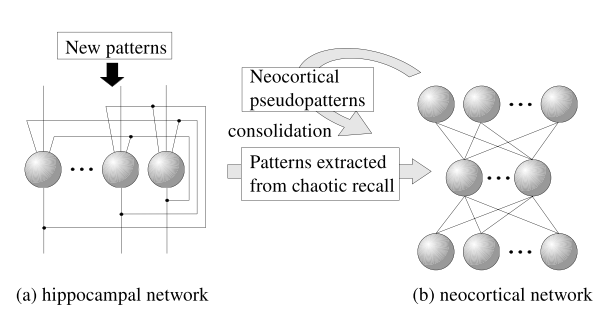
\includegraphics[width=10cm]{fig/hattori2010_model_structure}
\caption{An illustration from the paper of \cite{Hattori2010} of the proposed model. (a) represents the hippocampal module, whereas (b) represents the neocortical module. Note that the hippocampal module implements a Hopfield network, from which seemingly chaotic behaviour emerges when combined with the neuronal dynamics.}
\label{fig:hattori2010_model_structure}
\end{figure}

As can be seen from figure \ref{fig:hattori2010_model_structure}, \cite{Hattori2010} proposes a model in which the hippocampal (HPC) module is a single layer Hopfield network. However, the HPC module is not trained using gradient descent, but rather by Hebbian learning, which may be summarised as; fire together, wire together. Using Hebbian learning leads to faster convergence when compared to SGD \citep{Hattori2010}. Adopting \citeauthor{Hattori2010}'s (\citeyear{Hattori2010}) notation, the model may be formally outlined as follows, beginning with the equation for Hebbian learning;

\begin{equation}\label{hattori_hebbian_learning}
    \omega_{i,j}(t+1) = \gamma \omega_{i,j}(t) + x_i^{(k)} x_j^{(k)},
\end{equation}

where $\omega_{i,j}(t+1)$ is the weight between neurons $i$ and $j$ for time step $t+1$, $\gamma$ is a constant forgetting factor, $\gamma \in (0, 1)$, and $\textbf{x}^{(k)} = (x_1^{(k)}, x_2^{(k)}, ..., x_N^{(k)})$ is the $k$-th pattern that we want the network to learn. Note that $\textbf{x}^{(k)} \in \{-1,1\}^N$, which constrains $x_i^{(k)} x_j^{(k)} \in [-1,1] \implies \omega_{i,j} \in [-1-\gamma, 1+\gamma]$. $N$ is the number of nodes in the input patterns.

Further, \cite{Hattori2010} outlines the neuronal dynamics as follows;

\begin{equation}\label{hattori_next_output}
    u_j(t+1) = f\{\eta_j (t+1) + \zeta_j(t+1)\}
\end{equation}

\begin{equation}\label{hattori_former_inputs}
    \eta_j(t+1) = k_m \eta_j(t) + \sum_{i=1}^{N} \omega_{i,j} u_i(t)
\end{equation}

\begin{equation}\label{hattori_zeta}
    \zeta_j(t+1) = k_r \zeta_j(t) - \alpha u_j(t) + a_j
\end{equation}

Adopted to the thesis notation, $u_j$ is neuron $j$'s activation value, where the value for the next time step is determined by two functions, namely $\eta(t+1)$ and $\zeta(t+1)$. Equation \ref{hattori_former_inputs} takes into account its former input values through $\eta_j(t)$ for the current time step, in addition to summing over the inputs of its incoming synaptic connections. Equation \ref{hattori_zeta} includes a relationship to the neurons' previous activation values. Note that an external input parameter $a_j$ is also included in $\zeta_j(t+1)$, and that both equations \ref{hattori_former_inputs} and \ref{hattori_zeta} have damping factors of refractoriness $k_m$ and $k_r$, respectively, discontinuing the impact of former function-values exponentially relative to the temporal difference. $f(u)$ is the sigmoid function as defined in equation \ref{sigmoid}, note however that a steepness parameter $\epsilon$ is also included, $\theta$ being divided by $\epsilon$ such that,

\begin{center}
\begin{math}
    f(\theta) = \frac{1}{1 + e^{\frac{-\theta}{\epsilon}}}
\end{math}
\end{center}

% ====================================
\subsubsection{\cite{Hattori2014}}
\cite{Hattori2014} proposes a more biologically inspired dual-network memory model, based on and outperforming the model outlined above based on several experiments. In the novel model, \cite{Hattori2014} proposes a rather drastic architectural change in the hippocampal network, the neocortical module remaining the same. The hippocampal module is made out of five layers, the three middle layers being inspired by different parts of the hippocampus; namely the entorhinal cortex (EC), dentate gyrus (DG), and CA3, the first and last layer being the input and output layers. See figure \ref{fig:hattori_2014_model} for the topological structure of the novel model of \cite{Hattori2014}.

\begin{figure}
\centering
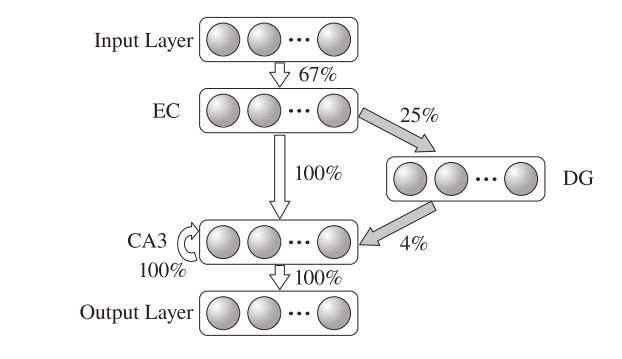
\includegraphics[width=10cm]{fig/hattori2014_hpc_module}
\caption{This figure by \cite{Hattori2014} illustrates his proposed dual-network memory model. Note that the EC is connected to both CA3 and DG, which in turn is also connected to CA3. The gray arrows are connections which are only used during training. Furthermore, CA3 is fully connected both recurrently as well as to the output layer. As EC is connected somewhat sparsely to the DG, and DG is very sparsely connected to CA3, this may constitute a form of compression mechanism as seen in auto-encoders. It is also worth noting that this poses a time-delay from when a certain input has been directly presented from the EC to CA3 until the possibly compressed input arrives from the DG. This may further constitute mechanisms similar to those of operating at multiple timescales, as well as mechanisms for abstraction.}
\label{fig:hattori_2014_model}
\end{figure}

It is worth mentioning that a slightly different transfer function is used by \cite{Hattori2014}. Namely,

\begin{center}
    $f(\theta) = tanh(\frac{\theta}{\epsilon})$,
\end{center}
where $\epsilon$ still is a steepness parameter.

Hebbian learning is still used as in equation \ref{hattori_hebbian_learning} for the CA3-layer and the CA3 to output-layer, relative to its former output;

\begin{center}
\begin{math}
    \omega_{i,j}(t+1) = \gamma \omega_{i,j}(t) + u_i u_j
\end{math}
\end{center}

However, between the EC and DG, EC and CA3, and DG and CA3 parts, Oja's rule is used (\cite{Hertz1991}, cited in \cite{Hattori2014}). Oja's learning rule is a modified type of Hebbian learning, restricting the weight space (to prevent divergence as a result of the chaotic behaviour). It may be formally outlined as follows,

\begin{equation}\label{ojas_rule}
    \omega_{i,j} = \omega_{i,j}(t) + \lambda u_j (u_i - u_j \omega_{i,j}(t)),
\end{equation}
where $\lambda$ is the learning rate for the Oja neurons. Note that the input and output layer neurons are bipolar ($\pm 1$), whereas the other neurons are binary. Every region is trained by a k-winners-take-all (kWTA) approach, in which a fixed number of the $k$ most active neurons' activation values are propagated throughout the neurons' synapses. Neuronal activity is determined by firing frequency. Interestingly, \citep{Hattori2014} notes that the non-linear separation of kWTA seems to be far more powerful than that of non-linear transfer functions. Furthermore, he notes that non-linear transfer functions may actually reduce the performance of kWTA.

One of the final keys to attaining a successful dual-network memory model introduced by \cite{Hattori2014} is neuronal turnover. Neuronal turnover is the birth and extinction of a percentage $\beta \%$ of the neurons, here in the DG. Note, however, that while this is believed to occur to a very low degree biologically in the DG, a very high rate of $\beta = 50 \%$ is employed by \cite{Hattori2014}, with turnover after every training set. Possible reasons for this and associated implications, related to plasticity and convergence, is discussed earlier in this section. \cite{Hattori2014} further demonstrates that the input patterns become less similar when introducing the neuronal turnover, which in turn drastically increases the number of patterns that may be stored in the HPC module.

Memory recall may be performed in the hippocampal network by chaotic recall after learning, i.e. presenting random input to the different sub-networks, waiting until it reaches some convergence criterion, considering the current pattern as a recalled memory. Another approach for interleaving new memories with old, as proposed by \cite{French1997}, is by re-instantiating the previously learned patterns from the neocortical module to the hippocampal network, thus interleaving everything contained in the neocortical network with a new hippocampal pattern. While biologically implausible and not that relevant for the current approach as outlined here, it is worth noting that a similar mechanism for re-instantiated a previously learned pattern to the hippocampal network if present in the neocortical network, might result in attaining novel abstract representations. This could resemble integration across memories more closely, and it is something I wish to further investigate in my future work.

\section{Notes}

Hodgkin-Huxley:

Would it be possible to fire using for instance 0.2 * sigmoid (in\_sum) for the neurons that do not fire 1?
\\\\

Approach topics that will be needed in the model and experiments.
Concepts
Terms
Definitions
Theory
Memory. Working memory.
The DNMA.
This chapter is essentially: Terms, definitions, concepts, papers, contemplations, background theory. Revisit DNMA.
Present previous model(s)?
Who are the reader..? A researcher with general knowledge within AI?

see notebook:

\begin{itemize}
    \item SLR DL \& CONN., including catastrophic forgetting in this context
    \item General (intro to) neuro. \& comp. neuro.
    \item + example
    \item may construct theories about brain function
    \item memory - largely connected to the hippocampus
    \item DNMA
    \item DNMA may solve catastrophic forgetting
\end{itemize}


\cleardoublepage